\chapter{Model implementation}

This chapter introduces the numerical implementation of the BTW sandpile model. Then we explain how the program is used to simulate the evolution of the sandpile system and avalanche behavior. Then, we deliver the analysis for the state of systems and avalanche properties. 



\section{Code Structure}

This project uses Python to implement the BTW sandpile model, and the program is designed according to the mathematical definitions in previous chapter. The code structure mainly consists of three parts: the core model class, the simulation control module, and the statistical analysis module. 

First, we use the \textit{SandPile} class to implement the main rules of the BTW model, including sand addition, toppling dynamics, boundary dissipation, and avalanche process. The function \textit{drop\_sand()} is used to add sand grains onto the lattice; the function \textit{topple()} performs the toppling process for the unstable site; the function \textit{avalanche()} repeatedly processes unstable sites until the whole system becomes stable; and the function \textit{avalanche\_length()} computes the avalanche radius. Further more, function \textit{mass()} and function \textit{is\_stable()} are used to monitor the system state. 

Second, we use the function \textit{run\_sandpile()} to perform the complete simulation procedure. This function controls the initialization for the lattice, setting and the random seed, and performs the burn-in process, then deliver the sampling simulation. During the burn-in process, the it adds sand grains and performs avalanche relaxation without recording statistical observables. During the sampling process, it records avalanche observables for the following statistical analysis.

Finally, the program contains functions for statistical analysis. The function \textit{plot\_average\_height()} is used to analyze the evolution of the average height and study the statistically stationary state. The function \textit{plot\_powerlaw\_distribution()} is used to fit the power-law distributions. The function \textit{plot\_gamma\_distribution()} is used to fit the gamma distributions. The function \textit{plot\_correlation()} is used to analyze the statistical correlations between different avalanche properties.



\section{Steady-State Behaviour}

In order to study whether the BTW sandpile model reaches a stable state, we investigate the evolution of the average height of the system. The average height \citep{Project2020} is defined as:

$$
\langle p_t \rangle
=
\frac{1}{NM}
\sum_{i,j} p_t(i,j),
$$

where $p_t(i,j)$ represents the number of sand grains at lattice site $(i,j)$ at time step $t$.

Before simulating, we first give a simple guess about the behavior of $\langle p_t \rangle$. Since the lattice is initially empty, then very few sands leave the system through the boundary at the beginning. As sand grains are continuously added onto the lattice, the total mass of the system increases, then the average height is expected to increase at the early stage. However, as sand grains accumulate on the lattice, more sites reach the instability threshold and produce the avalanche. Then the boundary loss gradually increases, and the sand grains added into the system begin to balance with the sand grains leaving through the boundary. Therefore, we expect that the average height will not increase without limit, but approach a stable level and fluctuate around it.

To verify this behaviour, we use a two-dimensional lattice with $N=64$, and perform $100000$ sand addition steps. During this simulation, the system keeps performing grain addition and avalanche relaxation, while recording the average height at each time step. Figure \ref{fig:ave_height_overtime} shows the evolution of the average height over time. At the beginning of this simulation, the average height increases rapidly. As the simulation continues, the average height reaches a level around $2.1$, and then fluctuates around it instead of increasing without limit. This result shows that the system can gradually reach a steady state. In this state, the system still changes because avalanche processes and boundary losses continue to occur, but overall it remains relatively stable. (\textbf{Ans. to Q4})

\begin{figure}[htbp]
    \centering
    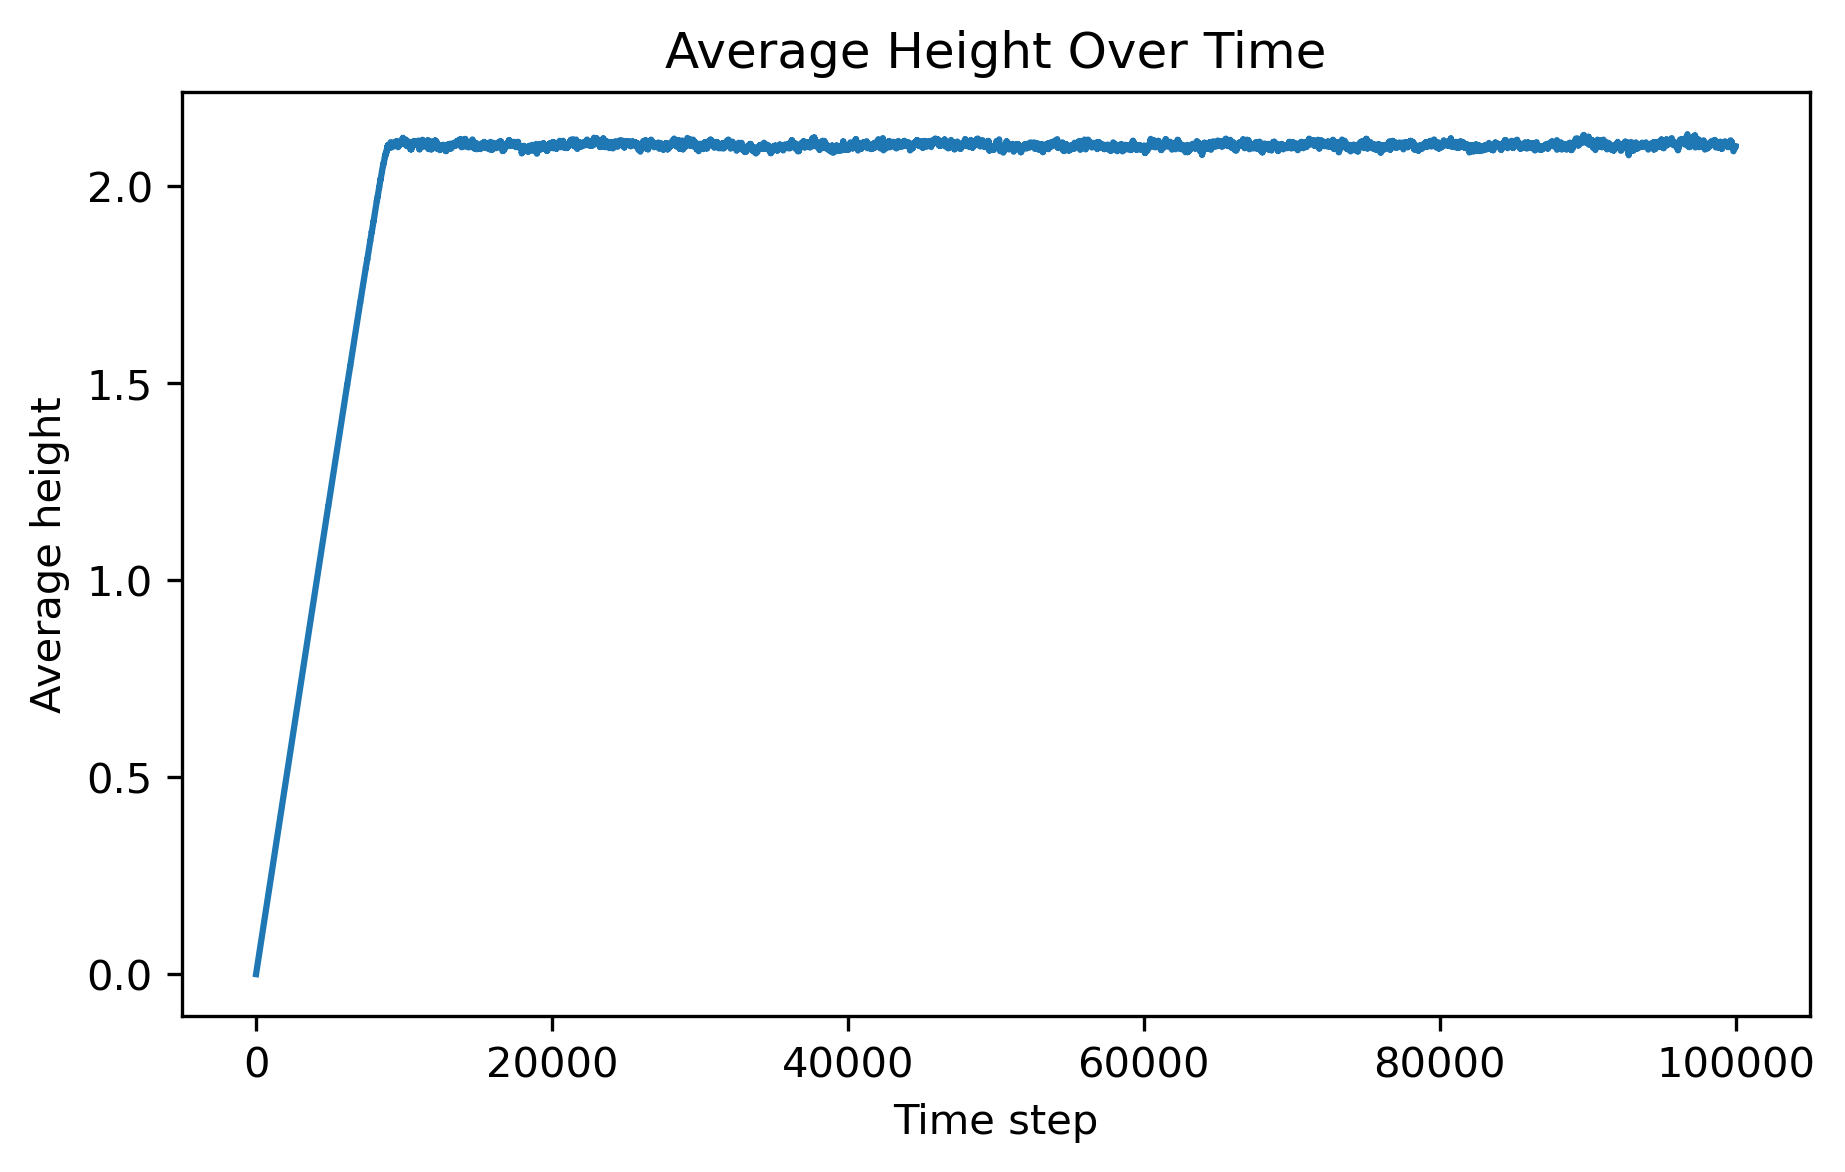
\includegraphics[width=0.6\textwidth]{figures/Ave_height_overtime.png}
    \caption{Average height over time}
    \label{fig:ave_height_overtime}
\end{figure}

Although the average height becomes stable after a sufficiently long time, we should distinguish different types of stability. In this project, it is important to distinguish between a steady state, a statistically stationary state, and an equilibrium state: The steady state means that some macroscopic observables remain approximately constant over time; A statistically stationary state means that, although the microscopic configuration of the system continues changing, the statistical properties of the system remain stable over time; An equilibrium state is different from the two states above. In an equilibrium system, there is usually no continuous external driving force or dissipation process. 

In this project, the statistically stationary state is mainly characterized by the behaviour of system observables. For example, the $\langle p_t \rangle$ fluctuates around a stable level after the initial growth stage, without showing long-term divergence. This behaviour indicates that the system could reach a statistically stationary state. (\textbf{Ans. to Q5})



\section{Avalanche Statistics and Correlations}

Before studying avalanche statistics, it is necessary to choose a reasonable the sampling method. For complex systems, sampling a system over time and sampling an ensemble of systems are not always equivalent. Sampling a system over time means evolving the same system for a long time and continuously recording the system observables. In contrast, sampling an ensemble of systems means considering many independent systems with different initial conditions, and then averaging their statistical quantities. If the system behaviour depends on the initial condition for a long time, time sampling and ensemble sampling may give different statistical results.

To discuss whether these two sampling methods are equivalent, we need to introduce ergodicity. If a system is ergodic, then after sufficiently long time evolution, its time average will approach the ensemble average:
$$
\text{time average} \approx \text{ensemble average}.
$$
For the BTW sandpile model, we consider that the system is approximately ergodic. First, the system continuously performs grain addition and boundary dissipation, so the lattice configuration keeps changing. Second, after the burn-in stage, the dependence on the initial condition becomes much weaker, and the average height and avalanche activity gradually enter a statistically stationary state. (\textbf{Ans. to Q6})

Therefore, this project uses time sampling to analyze avalanche statistics. In particular, after the burn-in process, the program continues running a single BTW sandpile system and records avalanche observables for the following statistical analysis. Then we study the statistical distributions of avalanche observables. The simulation uses a lattice with $N=64$, and records $200000$ avalanches after the burn-in process. The recorded observables are $(s,a,l,r)$.

Figure \ref{fig:topples_area_fit} show the distributions of avalanche topples $s$ and area $a$. The results show that these two variables are approximately linear on log-log plots, then we can fit them by using the power-law distribution, which is given by:
$$
P(x) \propto x^{-\alpha},
$$
where $\alpha$ is the power-law exponent. According to the fitting results, the exponent for topples $s$ is approximately:
$$
\alpha_s = 1.070,
$$
and the exponent for area $a$ is approximately:
$$
\alpha_a = 1.059.
$$

\begin{figure}[htbp]
    \centering

    \begin{subfigure}{0.40\textwidth}
        \centering
        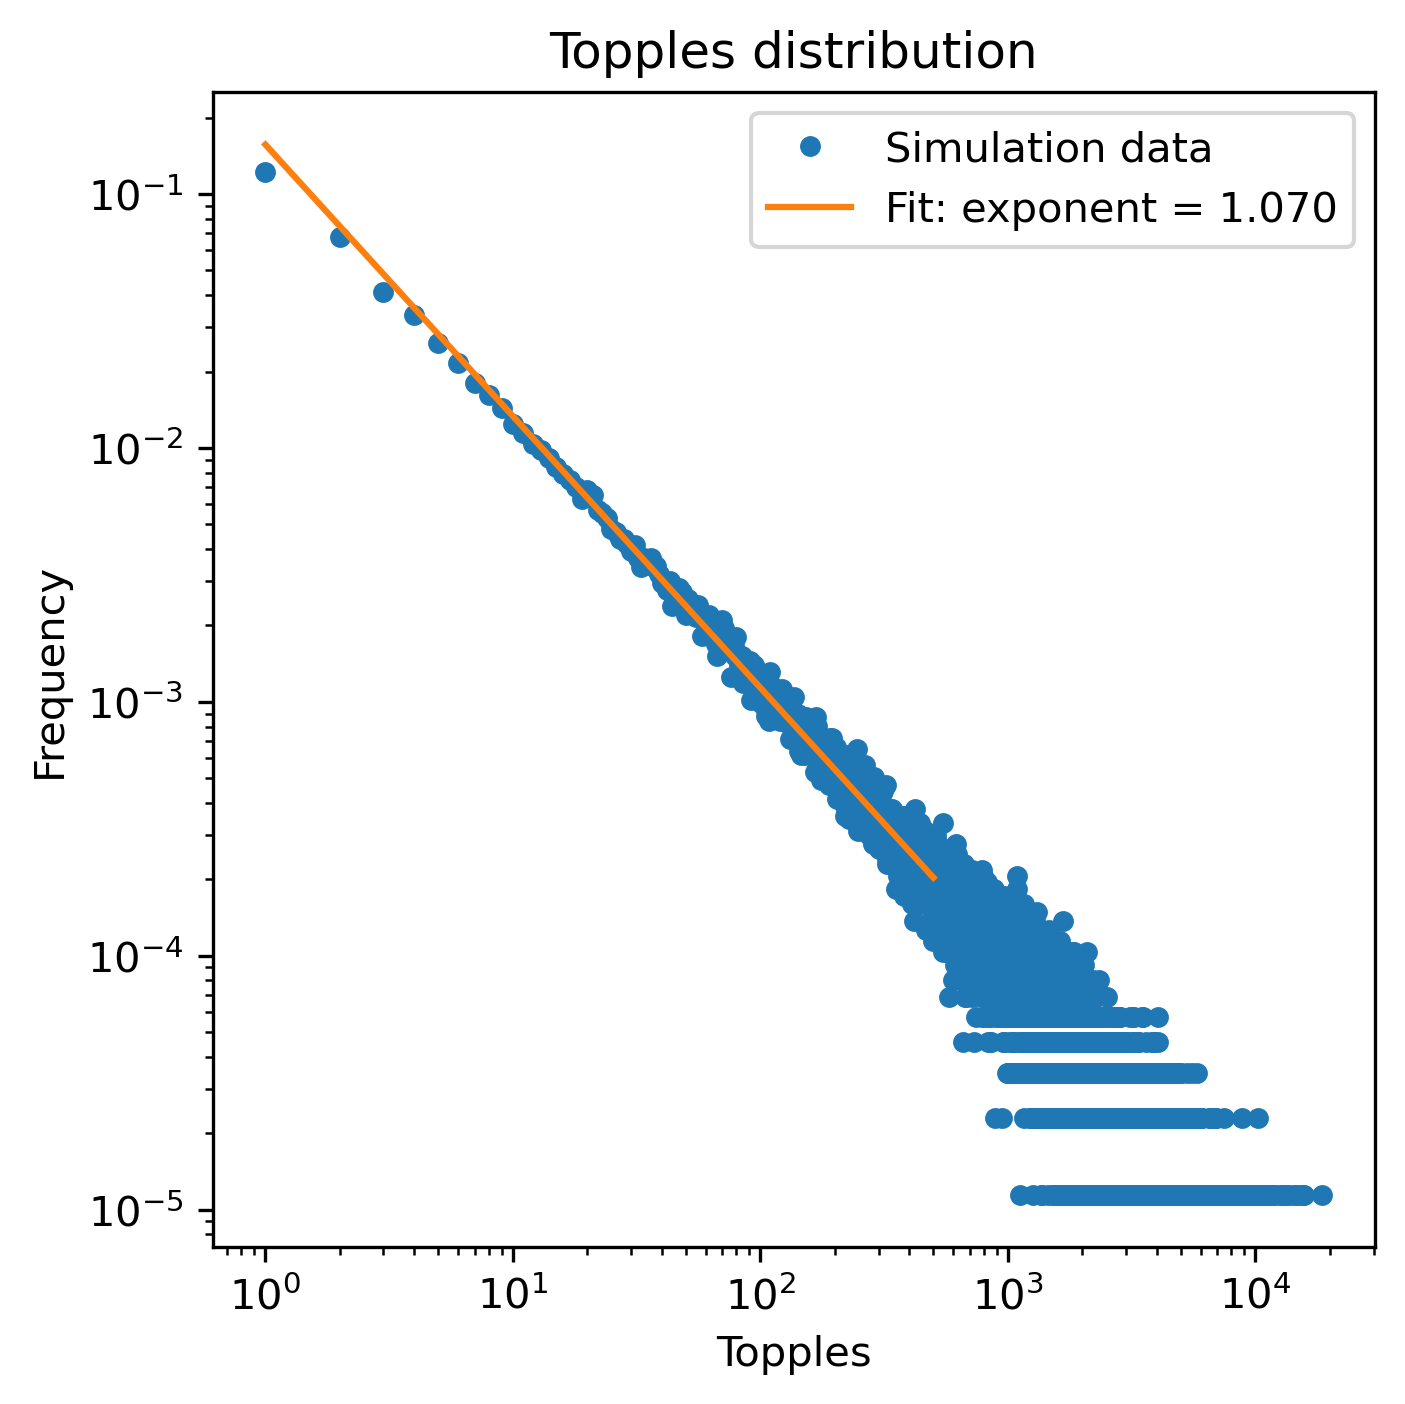
\includegraphics[width=\textwidth]{figures/topples_fit.png}
        \caption{Topples distribution}
        \label{fig:topples_fit}
    \end{subfigure}
    \hspace{0.06\textwidth}
    \begin{subfigure}{0.40\textwidth}
        \centering
        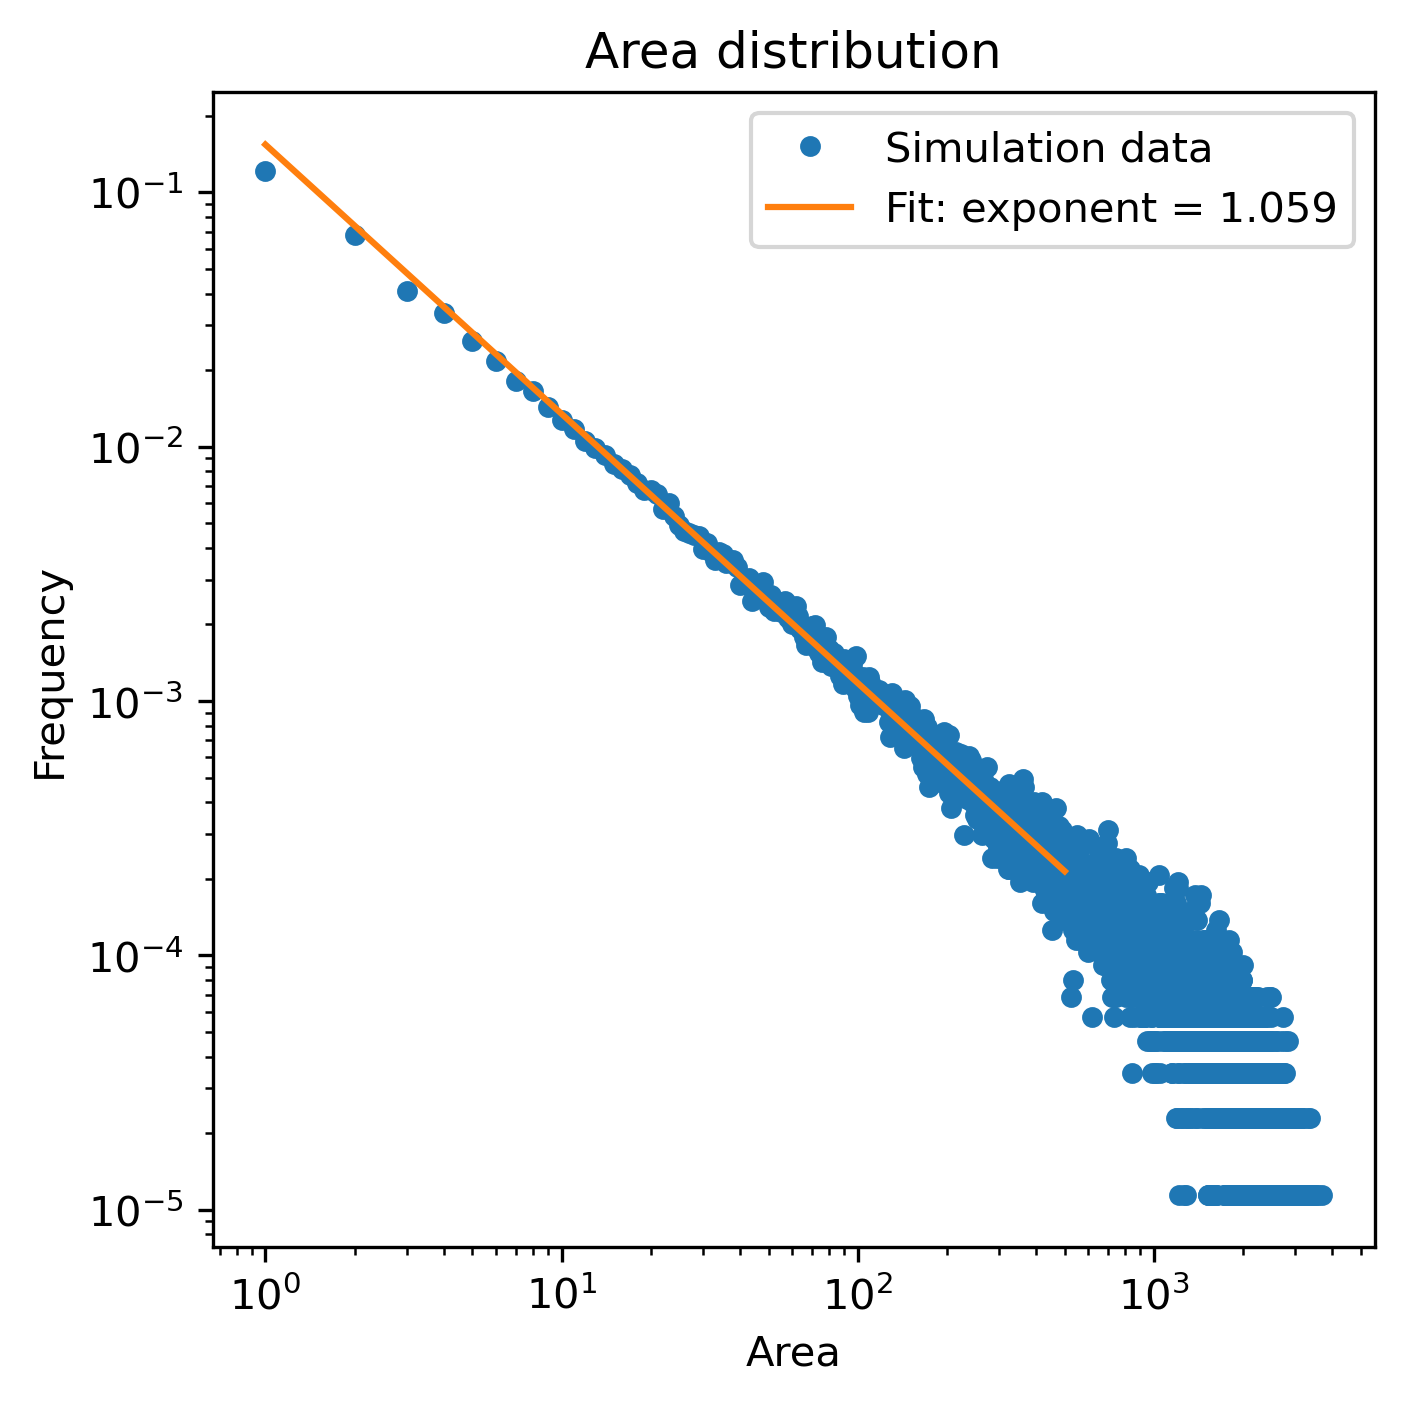
\includegraphics[width=\textwidth]{figures/area_fit.png}
        \caption{Area distribution}
        \label{fig:area_fit}
    \end{subfigure}

    \caption{Distribution fit for topples and area}
    \label{fig:topples_area_fit}
\end{figure}

In contrast, the distributions of loss $l$ and radius $r$ do not show very clear power-law behaviour. Then we consider using the Gamma distribution to fit them, as shown in Figure \ref{fig:loss_length_fit}. The probability density function of the Gamma distribution can be written as:
$$
f(x;k,\theta)
=
\frac{x^{k-1}e^{-x/\theta}}{\Gamma(k)\theta^k},
\qquad x>0,
$$
where $k$ is the shape parameter and $\theta$ is the scale parameter. According to the fitting results, the parameters for loss \(l\) are:
$$
k_l = 1.279,
\qquad
\theta_l = 4.904,
$$
and the parameters for radius \(r\) are:
$$
k_r = 0.930,
\qquad
\theta_r = 15.090. \quad (\textbf{Ans. to Q7})
$$

\begin{figure}[htbp]
    \centering

    \begin{subfigure}{0.40\textwidth}
        \centering
        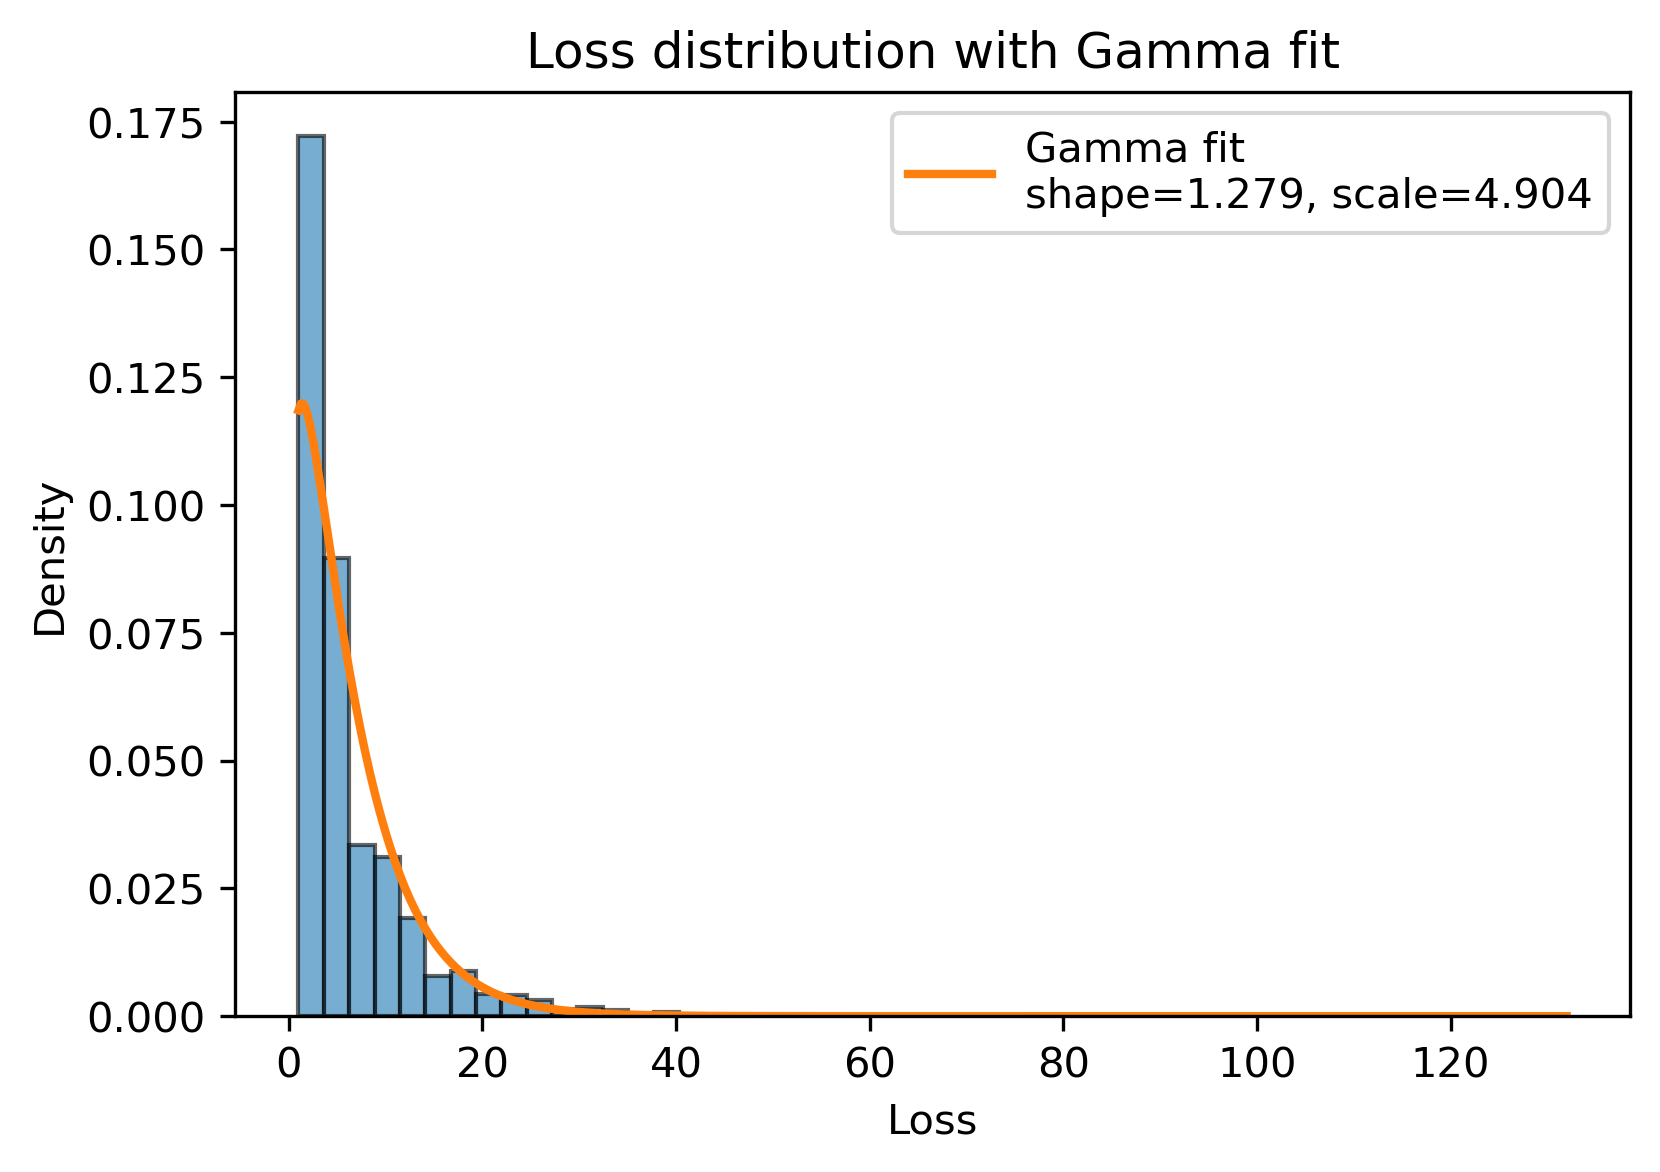
\includegraphics[width=\textwidth]{figures/loss_fit.png}
        \caption{Loss distribution}
        \label{fig:loss_fit}
    \end{subfigure}
    \hspace{0.06\textwidth}
    \begin{subfigure}{0.40\textwidth}
        \centering
        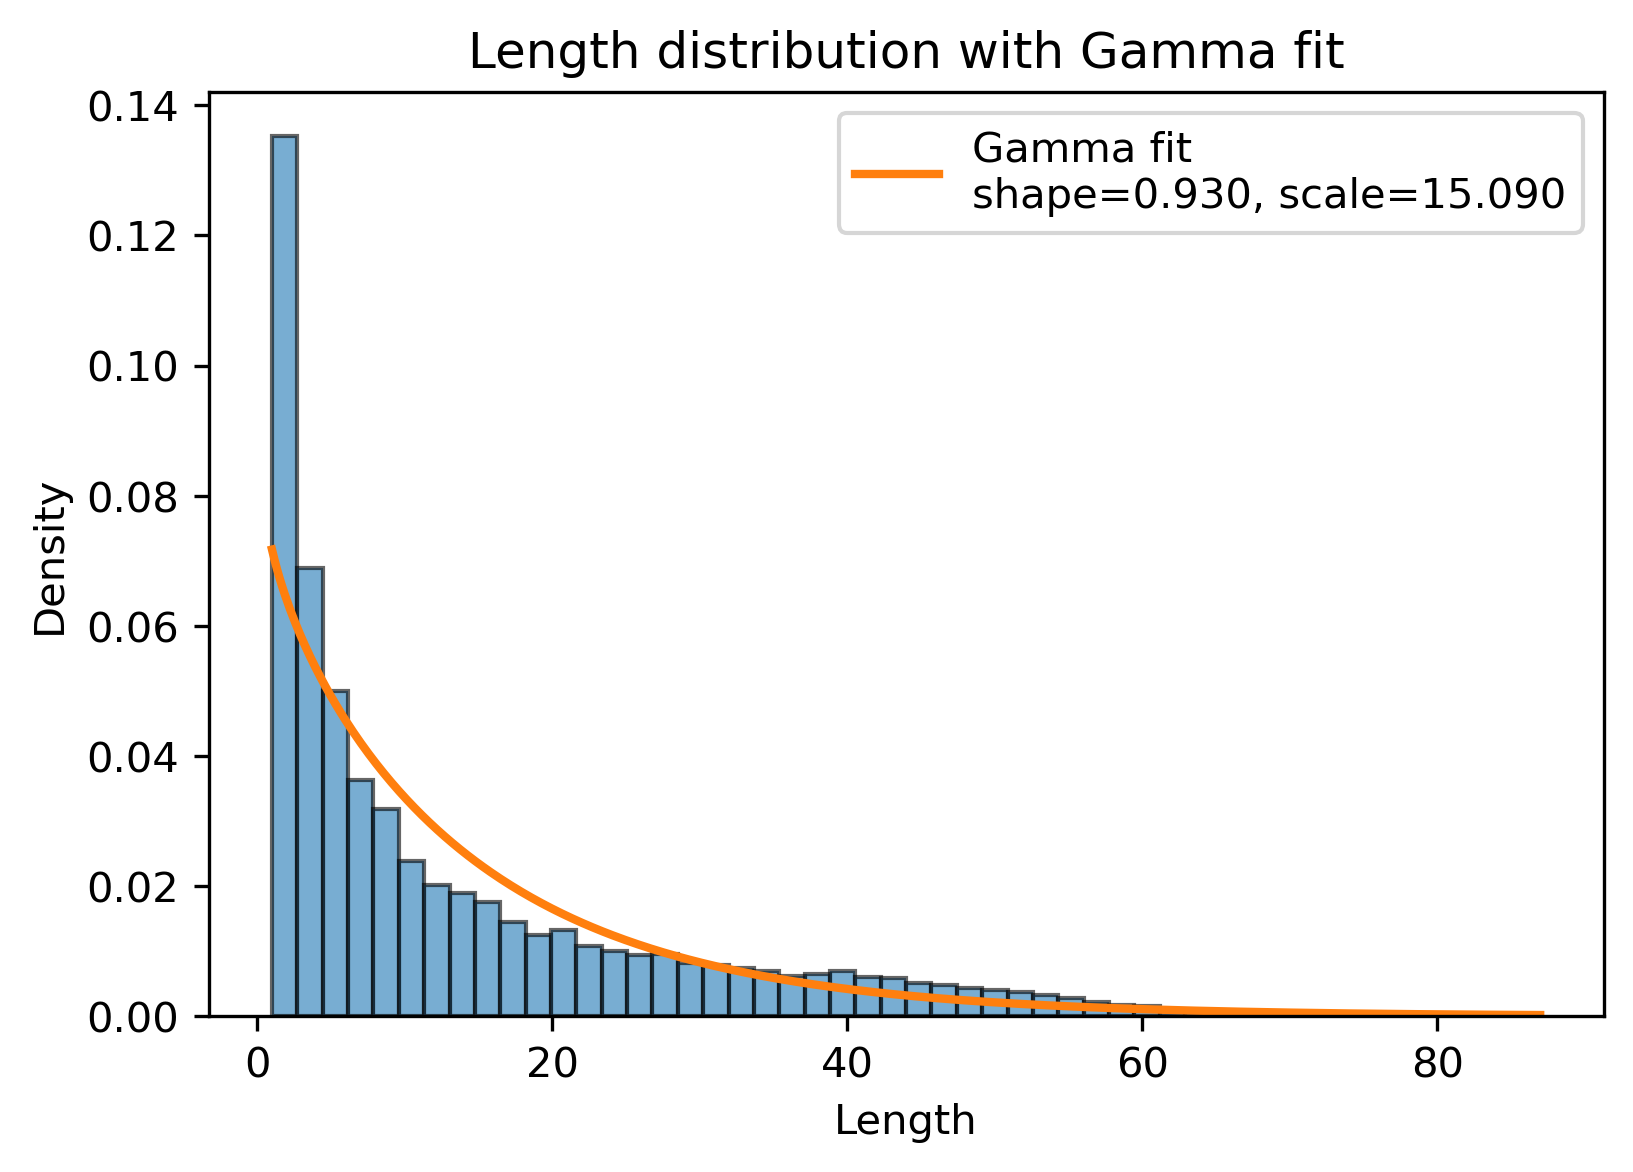
\includegraphics[width=\textwidth]{figures/length_fit.png}
        \caption{Length distribution}
        \label{fig:length_fit}
    \end{subfigure}

    \caption{Distribution fit for topples and area}
    \label{fig:loss_length_fit}
\end{figure}

Between the avalanche properties, We initially expect that $s$, $a$, and $r$ should show clear positive correlations. The reason is that a larger avalanche contains more toppling events, then it is more likely to affect more lattice sites, which can produce a larger avalanche area. At the same time, as the avalanche spreads farther across the lattice, the avalanche radius also becomes larger. 

The simulation results are shown in Figure \ref{fig: prop_high_posi_cor}, and they show agreement with the initial expectation --- the correlation coefficients for topples \& area and area \& length are $0.926$ and $0.890$, respectively. Furthermore, topples \& loss and topples \& length also show relatively strong positive correlations which are $0.736$ and $0.733$ respectively. It indicates that avalanches with more toppling events are more likely to reach the lattice boundary and to spread far away with the dropping site, then produce larger boundary loss and length. (\textbf{Ans. to Q8})

\begin{figure}[htbp]
    \centering

    \begin{subfigure}{0.40\textwidth}
        \centering
        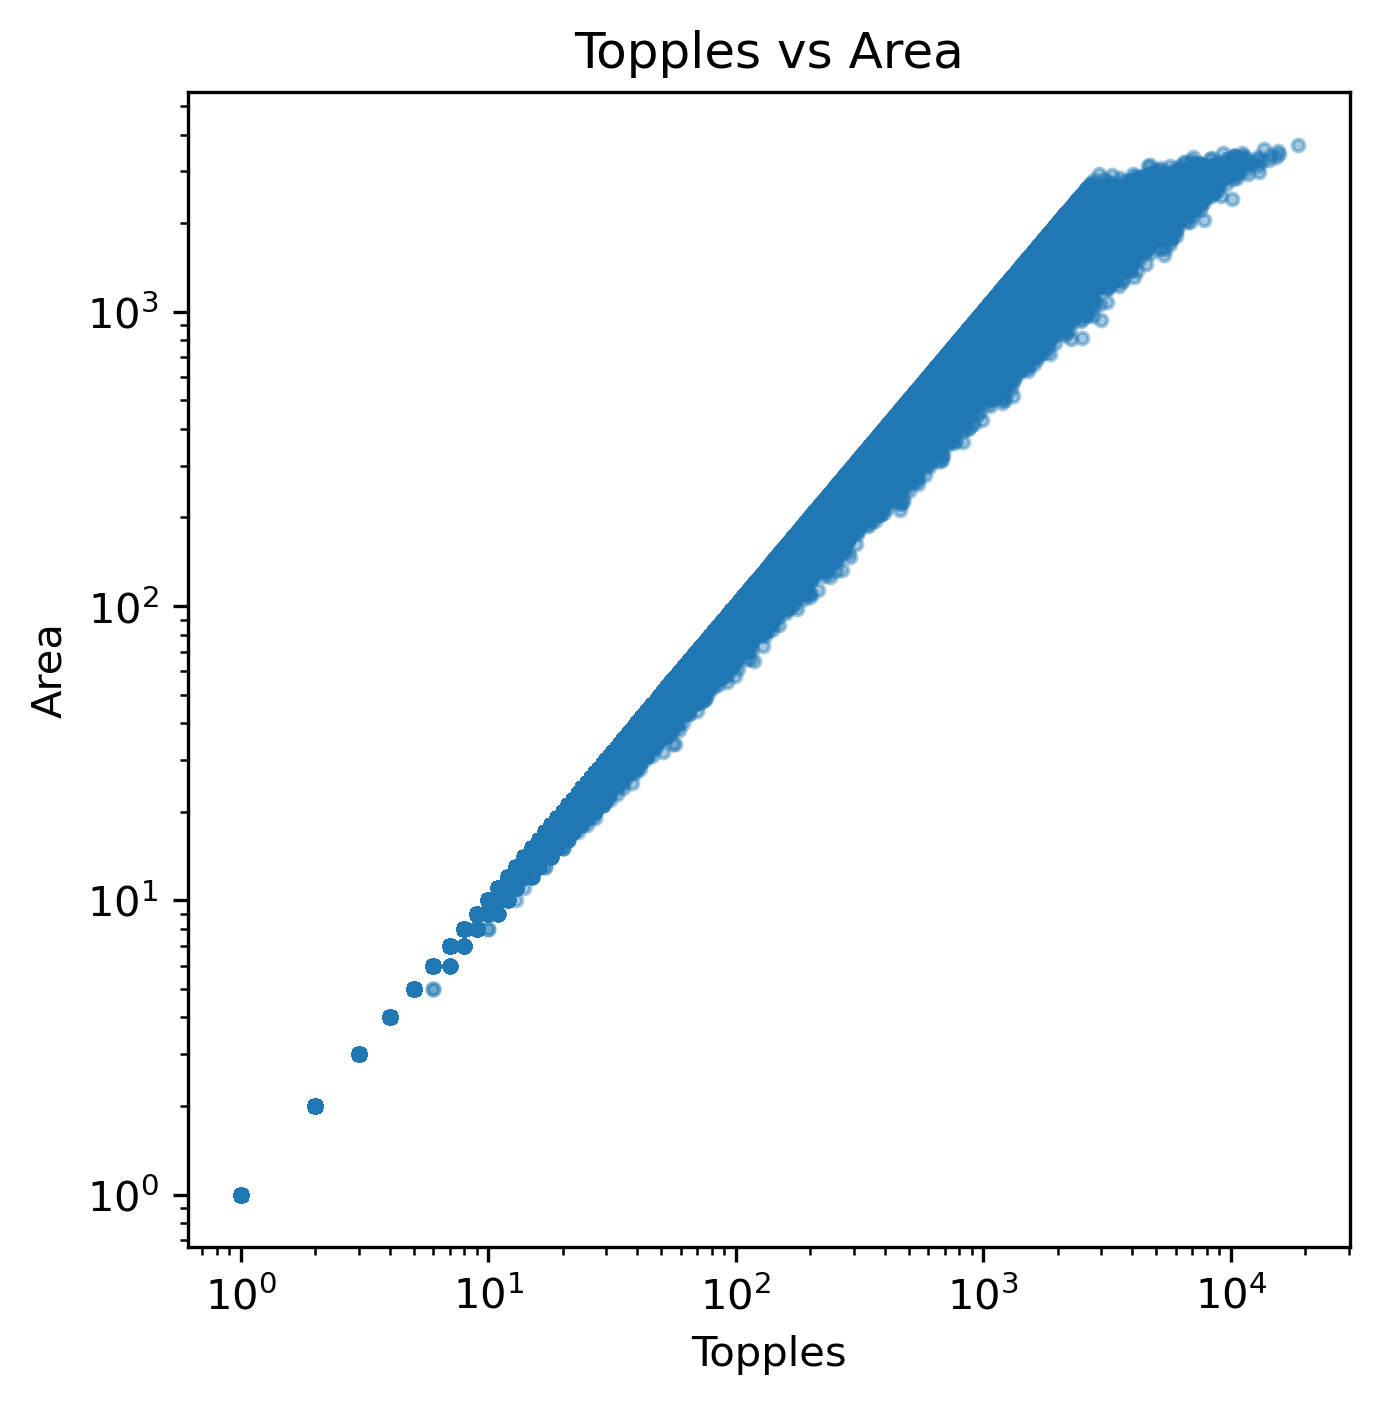
\includegraphics[width=\textwidth]{figures/topples_vs_area.png}
        \caption{Topples vs Area}
        \label{fig:topples_vs_area}
    \end{subfigure}
    \hspace{0.06\textwidth}
    \begin{subfigure}{0.40\textwidth}
        \centering
        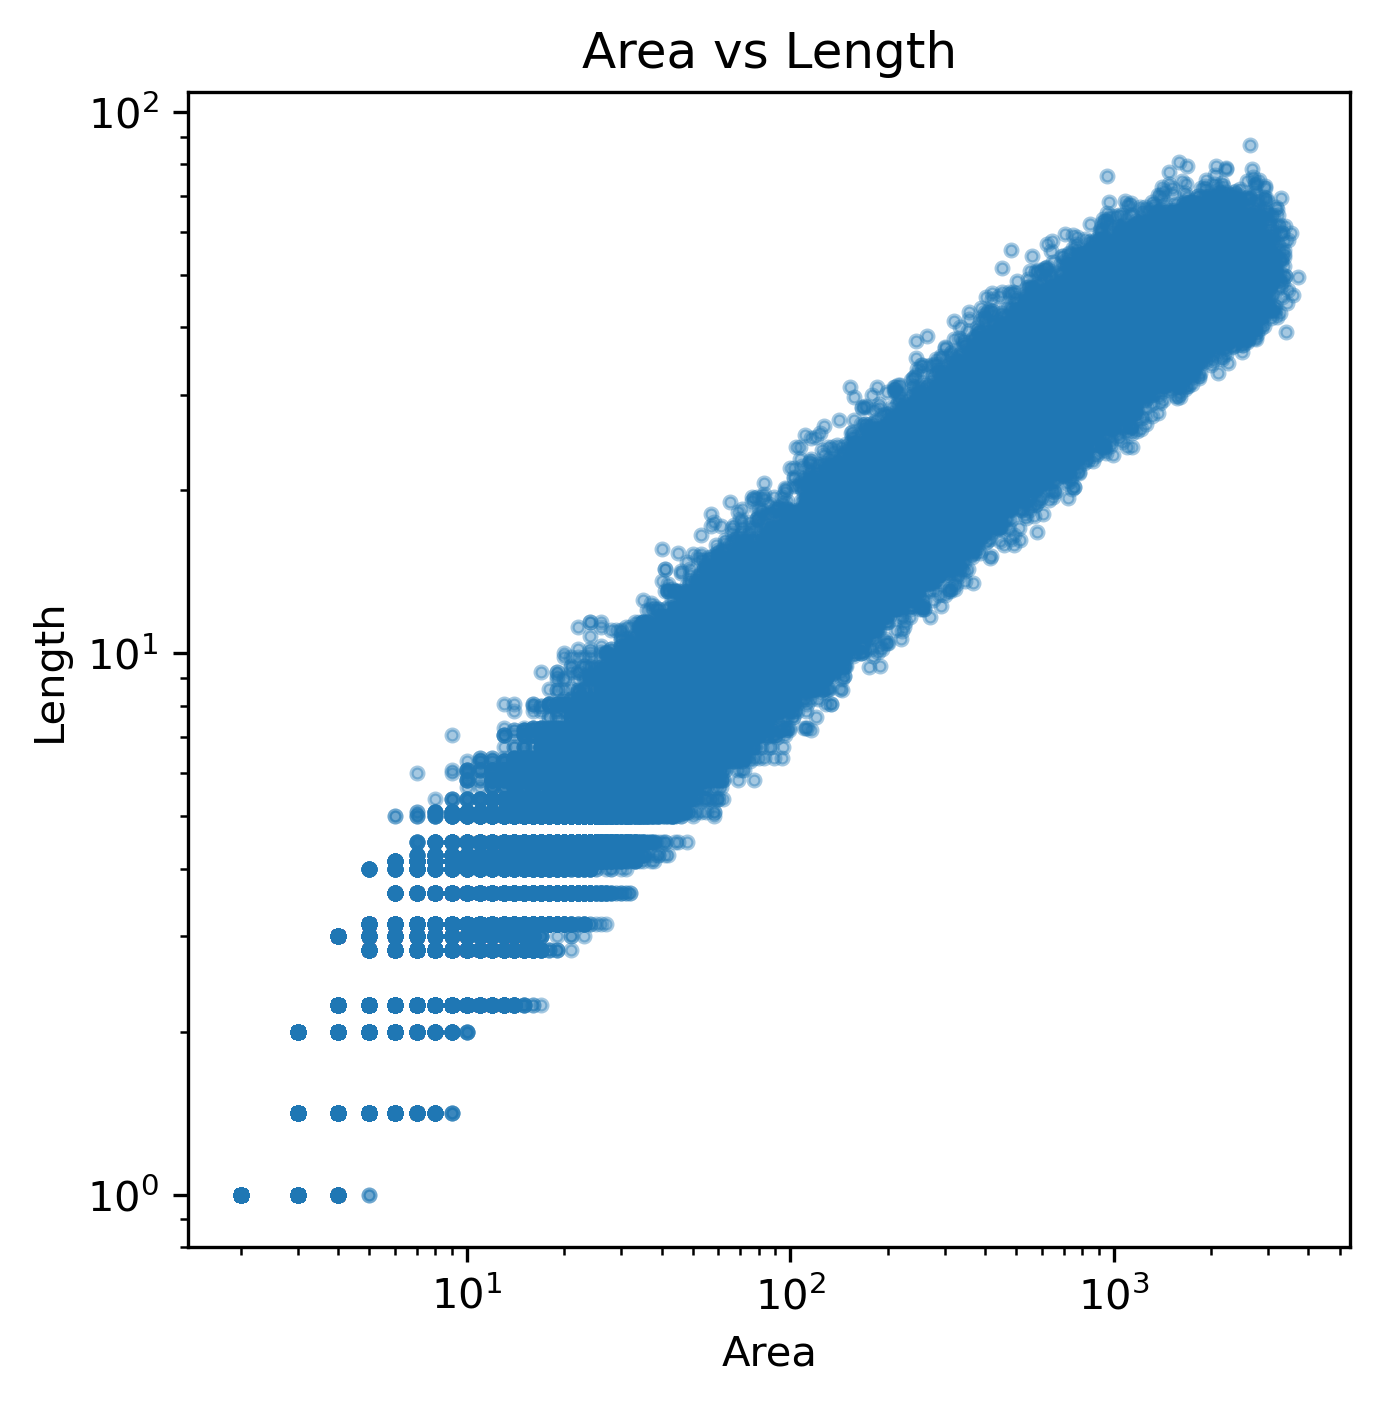
\includegraphics[width=\textwidth]{figures/area_vs_length.png}
        \caption{Area vs Length}
        \label{area_vs_length}
    \end{subfigure}

    \caption{Properties with high positive correlation}
    \label{fig: prop_high_posi_cor}
\end{figure}